% MIT License

% Copyright (c) [2023] [Eduardo Toledo Campos] [eduardotcampos@usp.br]

% Thanks to original latex timeline code creator claudio.fiandrino@gmail.com 

% Github https://github.com/cfiandra/timeline tikzlibrarytimeline.code.tex moved to the timeline
% diagram folder, the github also contains timeline example of latex file

% Timeline has been defined like the timespan is week (the default), and then a custom interval
% is set, considering the real timespan (or steps) desired

% Chemformula and chemfig packages used in chemistry writings and drawings, can be removed if
% this 2 elements are not desired

% \setchemfig is defined to set the chemistry drawings size

% Chemistry drawing are created by converting a .mol molecule file by the mol2chemfigPy3 python
% package, available in pypi and in https://github.com/Augus1999/mol2chemfigPy3

% Thanks to Augus1999 mol2chemfigPy3 creator

% The generated pdf file will be inserted in the main latex slides


%###################%
% Starting packages %
%###################%


\documentclass[aspectratio=169, border=0.1pt]{standalone}
\usepackage{xcolor}
\usepackage{tikz}
\usetikzlibrary{timeline}
\usepackage{chemformula}
\usepackage{chemfig}
\setchemfig{atom sep=2.25em}
\usepackage{helvet}
\begin{document}
\begin{tikzpicture}[timespan={}]
%---------------------------------------------------------


%##################%
% Timeline palette %
%##################%

% Good contrasts in white

\definecolor{tlred}{HTML}{DF0233}  % good contrast in white 
\definecolor{tlpurple}{HTML}{6112A4}  % perfect contrast in white
\definecolor{contrastgreen}{HTML}{00540D}  % perfect contrast in white  
\definecolor{contrastdarkred}{HTML}{960002}  % perfect contrast in white  
\definecolor{contrastbluegreen}{HTML}{0B5865}  % perfect contrast in white 
\definecolor{contrastpink}{HTML}{A10196}  % perfect contrast in white 
%----------------------------------------------------------------------------------


%##########%
% Interval %
%##########%

\timeline[custom interval=true]{MOF synthesis, NP synthesis, NP support, MOF $\ch{O2}$ binding, Application}
%----------------------------------------------------------------------------------------------


%########%
% Phases %
%########%

% The last phase and the phase before it are defined like they would be between the same
% phases, but one in the start of it (0.01) and one in the last of it (0.99), in the 
% pratice generating one phase in the last event and one phase in the event before it

% If the phase definition is desired to be between 2 of the timeline events, change the
% "in 0.01" to "in 0.5"

% The phase circle size is defined by the involvement degree 

\begin{phases}
\phase{between week=1 and 2 in 0.01,involvement degree=1.8cm,phase color=tlpurple}
\phase{between week=2 and 3 in 0.01,involvement degree=1.8cm,phase color=contrastgreen}
\phase{between week=3 and 4 in 0.01,involvement degree=1.8cm,phase color=tlred}
\phase{between week=4 and 5 in 0.01,involvement degree=1.8cm,phase color=contrastbluegreen}
\phase{between week=4 and 5 in 0.99,involvement degree=1.8cm,phase color=contrastpink}
\end{phases}


%############%
% Milestones %
%############%


% Síntese MOF

\addmilestone{at=phase-1.090,direction=90:1cm,text={\tiny\chemfig{[,.5]Zn-[:270.5,1.043]O-[:321.8,1.174](-[:42.6,1.072]O-[:90.5,1.043]Zn)-[:270]=^[:210]-[:270]=^[:330](-[:30]=^[:90]-[:150])-[:270]-[:210]-[:270]=^[:210]-[:270]=^[:330](-[:30]=^[:90]-[:150])-[:270]-[:225]O-[:270]Zn(-[:180]N)-[:270.8,0.911]O-[:315](-[:270,1.013]-[:330]=_[:270]-[:210](-[:270]-[:330]-[:270]-[:330]=_[:270](-[:41.3,9.3 ,,,draw=none]Zn)-[:210](-[:270](-[:218.2,1.174]O-[:268.5,1.043]Zn)-[:317.4,1.072]O-[:268.5,1.043]Zn)=_[:150]-[:90]=_[:30])=_[:150]-[:90]=_[:30])-[:45]O-[:90.8,0.911]Zn(-[:90]O-[:135])-[,1.163]N-[:300]=^-[:60](-[:120]=^[:180]-[:240]\phantom{N})--[:60]-=^[:300]-(-[:300]=_[:240]-[:180]=_[:120]-[:60])=^[:60](-[:120]=_[:180](-[:120]=_[:60]-=_[:300]-[:240])-[:240])--[:60]-=^[:300]-=^[:60](-)-[:120]=^[:180](-[:240])}}, text options={above}}
\addmilestone{at=phase-1.270,direction=270:2.6cm,text=\normalsize\textcolor{tlpurple}{Precursor 1 synthesis → Precursor 2 synthesis → MOF synthesis},text options={below}}


% Síntese NP

\addmilestone{at=phase-2.270,direction=270:1.8cm,text=\normalsize\textcolor{contrastgreen}{Gold, palladium, silver},text options={below}}
\addmilestone{at=phase-2.080,direction=90:2cm,text={\begin{tikzpicture}{\foreach \x in {0} \shade[ball color=green!\x0!yellow] (\x,0) circle (8mm);}\end{tikzpicture}},text options={above}}



% Suporte NP

\addmilestone{at=phase-3.285,direction=270:1cm,text=\normalsize\textcolor{tlred}{Best result nanoparticles},text options={below}}
\addmilestone{at=phase-3.080,direction=90:4cm,text={{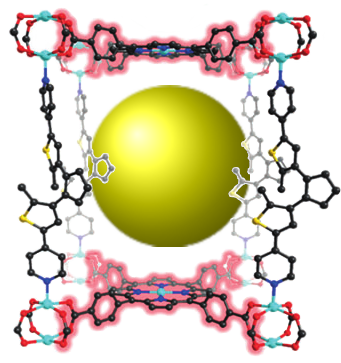
\includegraphics[width=3.4cm]{mofnp.png}}}, text options={above}}


% Ligação O2 MOF

\addmilestone{at=phase-4.285,direction=270:0.2cm,text=\normalsize\textcolor{contrastbluegreen}{342 nm irradiation},text options={below}}
\addmilestone{at=phase-4.080,direction=90:1.5cm,text={{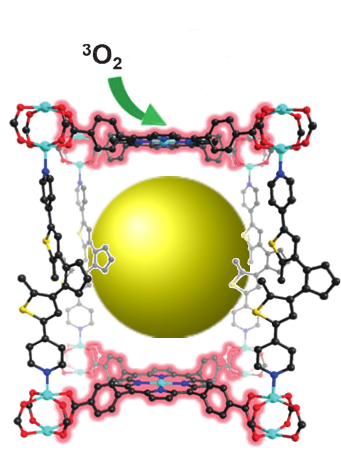
\includegraphics[width=3.4cm]{mofnpo2.png}}}, text options={above}}


% Aplicação

\addmilestone{at=phase-5.285,direction=270:1cm,text=\normalsize\textcolor{contrastpink}{Plasmonic region irradiation},text options={below}}
\addmilestone{at=phase-5.080,direction=90:4cm,text={{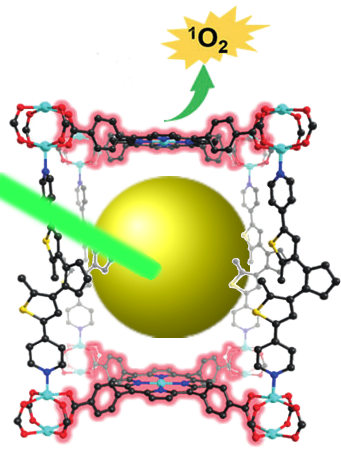
\includegraphics[width=3.4cm]{mofnpo1.png}}}, text options={above}}


\end{tikzpicture}

\end{document}
